\documentclass{article} 
\usepackage{apacite} 
\usepackage{graphicx} 
\usepackage{natbib}
\usepackage{listings}
\usepackage{epigraph} 
\usepackage{etoolbox} 
\usepackage{amsmath}

\usepackage{color}
\usepackage{array}
\newcolumntype{L}[1]{>{\raggedright\let\newline\\\arraybackslash\hspace{0pt}}m{#1}}

\definecolor{Red}{RGB}{255,0,0}
\newcommand{\red}[1]{\textcolor{Red}{#1}}  
  
\usepackage{listings}
%\usepackage{inconsolata}
\usepackage{xcolor} %to use colored text

%\lstset{
%language=Scheme,\lstinline
%basicstyle=\footnotesize\ttfamily,
%mathescape=true,
%frame=single
%}

\lstset{
  language=Scheme, % Andreas Stuhlmüller. Scheme listings. https://github.com/stuhlmueller/scheme-listings.git
  columns=fixed,
  tabsize=2,
  extendedchars=true,
  breaklines=true,
  frame=single,
%  numbers=left,
  numbersep=5pt,
    basicstyle=\scriptsize\ttfamily
%  rulesepcolor=\color{solarized@base03},
%  numberstyle=\tiny\color{solarized@base01},
%  keywordstyle=\color{solarized@green},
%  stringstyle=\color{solarized@cyan}\ttfamily,
%  identifierstyle=\color{blue},
%  commentstyle=\color{solarized@base01},
%  emphstyle=\color{solarized@red}
}

\makeatletter
\patchcmd{\epigraph}{\@epitext{#1}}{\itshape\@epitext{#1}}{}{}
\makeatother \def\signed
#1{{\leavevmode\unskip\nobreak\hfil\penalty50\hskip2em
\hbox{}\nobreak\hfil#1% \parfillskip=0pt \finalhyphendemerits=0
\endgraf}} \newsavebox\mybox \newenvironment{aquote}[1]
{\savebox\mybox{#1}\begin{quote}} {\signed{\usebox\mybox}\end{quote}}
\DeclareGraphicsExtensions{.pdf,.png,.jpg}
% Default margins are too wide all the way around. I reset them here
\setlength{\topmargin}{-.5in} \setlength{\textheight}{9in}
\setlength{\oddsidemargin}{.125in} \setlength{\textwidth}{6in}

\begin{document} \title{Motivated reasoning in minimal groups}
\author{Erik Brockbank, Andres Gomez Emilsson, and Michael Henry Tessler} \renewcommand{\today}{Psych 241\\June 8,
2014} \maketitle

\section{Introduction}

Research in motivated reasoning explores the intuitive idea that we are more likely to believe things we want to believe. While perhaps credible prima facie, any theory of reasoning as sensitive to motivation must account for the fact that most of us do not walk around in a world entirely of our own motivated fabrication. Classic findings in motivated reasoning establish the dynamic influence of our desires on cognition, inference, and reasoning while exploring the limits of the phenomenon--where it stems from and how it is constrained by competing goals of accuracy and accounting of evidence. In this paper, we discuss significant work in motivated reasoning and describe a set of experiments aimed at reproducing results from KK, hereafter ``KK'', with subjects on Mechanical Turk. We compare these results to a set of cognitive models programmed in the probabilistic language Church, which allows for quantitative comparison of the features of motivated reasoning. We raise critical issues for the motivated reasoning paradigm and discuss future directions for research in this area. 

\subsection{Background: Dissonance and Optimism}
Current theories about motivated reasoning emerged from earlier work on cognitive dissonance and optimism biases. Research done in the tradition of cognitive dissonance suggests some relationship between effort and subjective probability of events occuring. In \citet{Yaryan1961}, people who exerted energy memorizing lists in preparation for an uncertain future event (a ``pop-quiz") believed more strongly that the event would occur in comparison to subjects who only had to read over the lists in preparation. \citet{Arrowood1966} suggest the Yaryan and Festinger (1961) effect may in part be due to additional cues that the manipulation of effort may have afforded. In addition, they suggest the anticipation of effort expense is sufficient to manipulate subjective probability. They replicated the basic setup of Yaryan and Festinger (1961) with 110 (71 female) undergraduates. They used the same 6-point forced-choice scale which had no option for ``equal likelihood''. However, about 10\% of subjects responded with a write-in answer for ``equal likelihood''. Within the high anticipated effort group, 35 thought they would take the test they studied for, while only 14 thought they would take the other test, and 6 responded equal likelihood (64\%-25\%-11\%) vs. 23-28-1 (44\%-54\%-2\%). The participants were also instructed to write down the percentage of people present that would have to take the various tests (``objective probability''). Those estimates do not differ appreciably from 50\%-50\%. 

In a more contemporary literature, these findings may be referred to as the optimism bias, insofar as effort or expected effort can be construed as a cost and the opportunity to demonstrate one?s ability can be construed as a reward. The term optimism bias is defined broadly as ``the tendency to think that risk is less for oneself than for one's peers'' \citet{Klein2002}. In this literature, there is a suggested association between the optimistic bias and perceived control over the future event in question. Within this space, \citet{Taylor1988} discuss results challenging the notion that ``accurate perceptions of the self, the world, and the future are essential for mental health''. In particular, they outline three trends in reasoning that contradict this notion of human psychology as consistently in tune with reality: unrealistically positive self-evaluations, exaggerated perceptions of control, and unrealistic optimism. All of these fall under what Taylor and Brown call a general pattern of positive self illusions. We will return to the ideas of overly-positive self-evaluation and unrealistic optimism in our own modeling, discussed below. Examples of the two are widespread in the literature. Regarding positive self-evaluation, \citet{Taylor1988} note that that people typically judge positive traits as more descriptive of themselves than negative traits, are better at recalling positive personality information or examples of success than negative information or examples of failure, and are more inclined to dismiss negative aspects of the self or the importance of things they are not proficient at. Results in optimism are similar. People estimate the likelihood of positive events happening to themselves in the future as far greater than the likelihood of such events happening to their peers, while their estimations for the likelihood of negative events are much lower for themselves than their peers; even in outcomes of chance, people find positive outcomes more likely and negative ones less so \citet{Taylor1988}. From these early results emerges a picture of human reasoning agents as frequently susceptible to the beliefs which suit them best, even when such beliefs run at odds with laws of probability or causality. 

\subsection{Motivated Reasoning}
The notion that we are, at least in certain reasoning contexts, likely to adopt the belief which coheres with a high-level tendency towards optimism and positive self-evaluation over the belief which more strictly attends to the demands of rationality forms the basis for research in motivated reasoning. In ``The Case for Motivated Reasoning'' \citet{Kunda1990}, Ziva Kunda proposes an underlying mechanism for this paradigm, namely that the motivation to arrive at a particular conclusion can lead us to adopt biased strategies for accessing, constructing, and evaluating beliefs which are most likely to support this conclusion. Critically, Kunda argues that this is a process constrained by the motivation to arrive at the conclusion which is most accurate; the idea that motivated inference is constrained by accuracy motivations is supported by work showing that increasing the need for accuracy through the threat of external evaluation, public display of one's judgments, or the possibility of having to defend them, reduces cognitive biases. On the flip side, Kunda argues that motivated reasoning occurs when the evidence for a desired conclusion is such that a dispassionate observer might be convinced of the conclusion---in other words, where we can sufficiently justify a desired belief, we are far more likely to adopt it even when doing so does not conform with the desire for accuracy. An array of evidence from research on cognitive biases and dissonance reviewed by Kunda suggests that beliefs about the self, beliefs about others, and beliefs about future outcomes, on the basis of certain kinds of evidence, will trend away from what is strictly accurate and towards what we would most like to believe. The key departure from earlier research on dissonance is the observation that across these areas of reasoning, the inconsistency between possible beliefs is accompanied by an inducement of motivation for one belief or another: it is the directional goals and not the inconsistency which causes the behavior. Kunda argues that future research in this domain ought to address the biased mechanisms of memory access, evidence, and evaluation which seem to support the formation of motivated beliefs. 
\section{Methodology: Prior Motivations and Minimal groups}
The goal of further dissecting the motivated reasoning process raises questions about how best to test hypotheses in this domain, drawing on and altering earlier paradigms in dissonance research. If we take the basic elements of motivated reasoning to be i.) the desire to arrive at a certain conclusion, ii.) a set of available conclusions in which the one desired is not necessarily consistent with the desire for accuracy, and iii.) some evidence on which we are asked to base a conclusion, experiments in motivated reasoning will control for some of these while manipulating others. Doing so raises certain methodological challenges, most notably the question of how best to generate the first component above in a way that allows for control and manipulation groups. Research on motivated cognition has taken two tacks at resolving this possible confound. The first is to select an issue around which we expect some people to have a pre-existing motivation, and the second is to induce motivation in artificial contexts. 
\subsection{Prior Motivation}
A clear example of the first strategy comes from a study by \citet{Bastardi2011} with participants who had indicated on a pre-survey that they thought home care was superior to day care. Of these participants, half expressed intentions of enrolling their children in day care--the ``conflicted'' group--despite the above convictions, presumably due to outside factors, and the other half expressed intentions of caring for their children at home--the ``unconflicted'' group--consistent with their beliefs about which was better. Accordingly, the conflicted group should be motivated to reason that day care is better (i.e. that their initial convictions were wrong). Participants were asked to read two fictional studies with distinct methodologies and with opposite conclusions (one that child care is better, the other that home care is better). Perhaps unsurprisingly, The conflicted group valued the study significantly higher when its results supported day care than home care; their evaluation was consistent with their motivations to justify the choice of day care despite their earlier misgivings. In the unconflicted group, participants rated the study more negatively when its results supported day care. This design and its results are typical of other research in motivated inference which selects participants with certain existing motivations in order to evaluate how such motivations affect subsequent inferences. These studies, however, have the problem of separating motivation from differences in prior beliefs (e.g. smokers may just believe smoking is not as bad as nonsmokers believe, even without taking into account motivation). The Bastardi study tries to get around this issue by only selecting participants who believed day care was indeed better than home care.
\subsection{Minimal Groups}
A second strategy in formalizing a motivated inference paradigm is to induce motivation, controlling for whether a participant is motivated to draw a certain conclusion (and potentially how much) by whether they receive a particular manipulation. This is commonly done with ``minimal groups'' paradigms, in which participants are assigned to be responsible for a particular cause or outcome in a made-up team game where they will be rewarded based on whether they win. KK used a typical structure for motivated inference research. In that study, 63 male Princeton undergraduates were told that they would be competing in an American History quiz game in which they would be partnered with a randomly selected teammate; the participant would be tasked with selecting questions from a list to give his teammate, who would then have to answer the questions. Teams would compete to answer the most questions and win 50 dollars. After being shown a sample set of quiz answers in which all questions had been answered correctly by a previous participant (ostensibly to provide the participants with a sense of what the questions were to look like), participants were told that the sample quiz had belonged to either (A) the participant's partner for the next round, (B) one of the participant's opponents on the next round, or (B) a previous participant not involved in this round (control). After being shown the sample quiz, participants responded to questions about the skill level of the person who took the sample quiz, the skill level of the average Princeton student, and the role of luck in the game. 
Consistent with the motivated inference hypotheses, participants who judged partners rated that person's ability as significantly higher than participants who judged opponents. In particular, partners rated the target person similarly to control subjects; the effect was driven by opponents, derogating the target. Additionally, opponents rated the average person's ability as significantly higher than partners and controls; if the average person is pretty good at the task, the opponent does not seem exceptional. Finally, opponents rated luck as being far more contributive to success in the game than partners (who rated it as lower than the control condition), again consistent with motivations among opponents to derogate the true ability of the target person and motivations among partners to elevate the target person's ability.  

Klein and Kunda attribute these findings to the theory that people placed in a teammate or opponent relationship with a target person will not only form motivated inferences about that person, but will also form more general motivated beliefs (about the average person's ability and the role of luck in the game) which allow them to further justify their beliefs about the target. Additionally, participants were placed in one of two ``degree of evidence'' conditions which varied the number of questions on the ``sample quiz'' (thus, the amount of evidence about the target). The effects described above were stronger for participants in the 2-question condition than the 8-question condition, indicating the extent to which motivation can act on reasoning is constrained by the available evidence (and presumably, an accuracy goal). Klein and Kunda's 1992 work (and the background literature described here) form the basis for our own research, which places Mechanical Turk users in a minimal group setting and, after providing some evidence about earlier results from another Turker, elicits judgments about the ability of this player, who is to be either the participant's teammate, opponent, or neither in the upcoming game. In what follows, we discuss computational models for this experiment as well as the empirical results.

\section{Two computational models}

We compose a generative model that considers an team game analogous to that used in KK. A game is made up of two teams playing in parallel to accrue points. A point in the game is a Bernoulli random variable that can be true in one of two ways: either by the team being skillful or by the team being lucky, as in:

\begin{lstlisting}
   (define (single-hit team type-of-game)
    (if (flip (luck type-of-game)) 
      (flip) 
      (flip (team-ability team))))
\end{lstlisting}

A team gets lucky according to probability 0.5 in situations where the point is determined by luck, this latter component is determined by \lstinline{(flip (luck type-of-game))}. This captures the intuition that some games have a lot of luck involved, whereas others are determined largely by chance. If the round is not determined by luck, then the team gets a hit in proportion to their teams abilities. 

Our game involves teams with distinct roles and as such, the \lstinline{team-ability} could be determined by the product of the individual players' abilities, as in:

\begin{lstlisting}
   (define (team-ability team)
     (prod (map (lambda (person) (player-ability person)) team)))
\end{lstlisting}

However, in the KK setup, as well as in ours below, there is reason to believe the roles are asymmetric. As well, using the product of the two players abilities to determine the probability of a correct answer makes the task more difficult than we would expect. This is important when we consider inferences about \lstinline{luck} later. For these reasons, our models consider the team's ability to be determined by only one player, as in:

\begin{lstlisting}
(define (team-ability team) (strength (first team)))
\end{lstlisting}

We consider a player's ability to a persistent, but random, property of the individual. We consider the luck in a game to be defined similarly. 

\begin{lstlisting}
   (define player-ability (mem (lambda (person) (ability-prior))))
   (define luck (mem (lambda (type-of-game) (luck-prior))))
\end{lstlisting}

We want the mean team performance to be approximately 50\%, so we define \lstinline{ability-prior} to be a \lstinline{(beta 3 1)} distribution (implicitly then, the team ability distribution is \lstinline{(* (beta 3 1) (beta 3 1))}. We take \lstinline{luck-prior} to be a symmetric \lstinline{(beta 3 3)} distribution. 

In KK, participants were given evidence about the past performance of a target individual. The evidence they received was in the form of \lstinline{total-hits}, which is defined as \lstinline{(repeat num-rounds (lambda ()   (single-hit team type-of-game)))}. Thus, the form of the evidence the participants received was:


\begin{lstlisting}
(condition (equal? (total-hits '(target other) 'history 8) 8))
\end{lstlisting}

This says that the total-hits of the target person in an game which had eight rounds was equal to 8. The reason \lstinline{'other} is included is because the game is a two-person game, and so even though the other player is not referred to explicitly in the evidence, she needs to be included to make sense of the \lstinline{total-hits} function. Notice also that the string \lstinline{'history} is used to signify that we are referring to a particular type of game (e.g. the history game). This is important in determining the value of \lstinline{(luck type-of-game)}, which we defined as a persistent property of a game.

The predictions of the base model in Figure \ref{fig:base}. Throughout this modeling section, we will show plots with bootstrapped 95\% confidence intervals for the following four quantities: (1) perceived ability of target (2) perceived ability of the average player (or, a randomly selected new player) (3) perceived luck in the game and (4) the probability of winning a game against a team that includes the target individual. 

\begin{figure}
\centering
    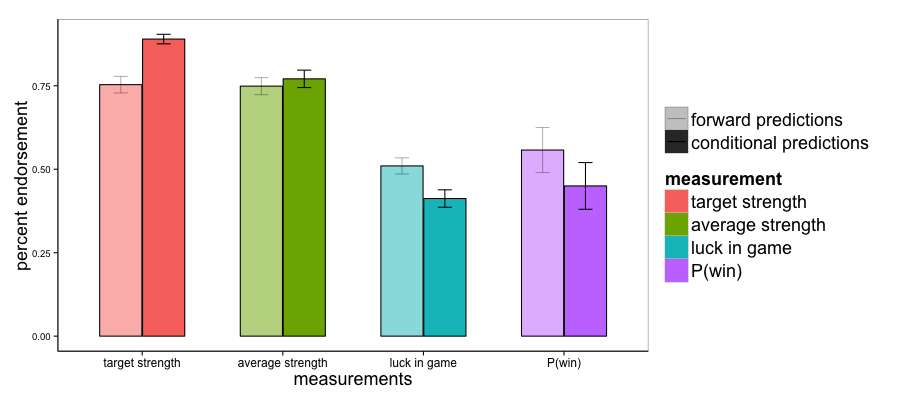
\includegraphics[width=\columnwidth]{basePredictions}
    \caption{Base model predictions. The forward predictions are simply the results of the generative model conditioned on no evidence. The conditional predictions are those conditioned on the target getting 8 out of 8 questions correct on the previous round.}
      \label{fig:base}
\end{figure}


Below, we consider two possible sources of motivated reasoning: optimism and perceived excellence. 
\subsection{Optimism model}

In the Optimism model (henceforth, Model O), the participant is optimistic about his expected performance in the upcoming match. This is implemented in the model by introducing a new conditioning statement: 

\begin{lstlisting}
(if (flip optimism) 
    (eq? 'team1 (match-winner my-team their-team game num-rounds)) 
    (eq? 'team2 (match-winner my-team their-team game num-rounds)))
\end{lstlisting}

This states with with a certain degree of optimism \lstinline{(flip optimism)}, the participant expects her team will win the next match. If \lstinline{optimism} is equal to 1, the state of the world is updated as if the participant has already won. If  \lstinline{optimism} is equal to 0, the participant believes with absolute certainty that she will lose. To account for the effects of KK, \lstinline{optimism} would fall between 0.5 and 1. 

In Figure \ref{fig:modelo}, we show below what happens when optimism is set to 1. We consider model predictions for the main experimental manipulation in KK: the role of the target. Predictions for when the target is the participant's partner, opponent, and control condition are considered when an optimistic outcome is assumed. The effects are subtle but robust. When considering the target ability (or target strength), the partner tends to overestimate and the opponent tends to underestimate the target's ability. The opposite is true for the role of luck in the game. 

One possible reason for the subtlety of the effects can be found in the difference between the evidence for the target and the optimistic outcome condition. We are given the target performance on individual trials (or questions): she gets 8 out of 8 correct. The optimistic outcome, however, is about the match-winner. The condition is that we get more questions correct than our opponent. This is a weaker condition that the evidence about the target. For example, it's possible to achieve this condition with the target's team getting 7 out of 8 correct in our hypothetical optimistic game, and so the evidence is not so strong against the idea that the target has considerably high ability. 

\begin{figure}
\centering
    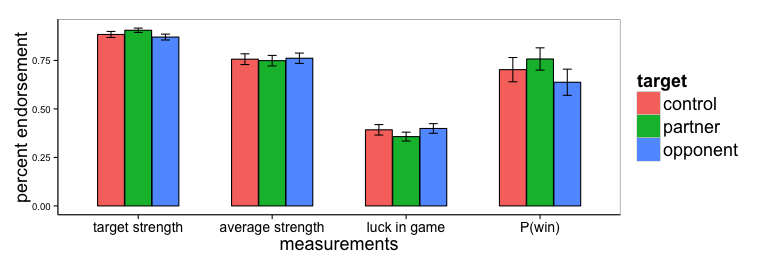
\includegraphics[width=\columnwidth]{modelO-predictions}
    \caption{Model O predictions. ``Target" refers to the main experimental manipulation in KK. Partner or opponent refers the target individual's relationship to the participant in the upcoming round. In the control condition, the participant rated an individual who was neither going to be their partner nor opponent.}
      \label{fig:modelo}
\end{figure}


\subsection{Excellence model}
In the Excellence model (model E), the participant does not have optimistic (or pessimistic) expectations about the future but rather believes she is an above average player. This would also lead to a ``better than expected'' performance at the game (meaning that the probability that her team will win is better than the evidence would suggest). For this we need to assume that the participant is uncertain about what the average ability is (or, equivalently, how difficult the game is), but knows that whatever the average is, she is better than it.

For simplicity, we randomly sample the \lstinline{alpha} parameter of the beta distribution and for simplicity, we take
\lstinline{(define alpha (uniform-draw (list 2 3 4 5 6)))}. This corresponds to the difficulty of the task (or likewise, the average ability). The higher the alpha the easier the task. To adequately compare across models, we assume the \lstinline{mean-strength} is subtracted from the target strength and \lstinline{0.75} --- the mean in the base model --- is added back, as in \lstinline{(+ (- (strength 'target) mean-strength) 0.75)}.

The influence on the experimental queries is a little more subtle in this model, but it seems that the both Model O and Model E make the same predictions about the appraisal of target strength. The models appear to diverge in their predictions about the ability of the average person in the game.

\begin{figure}
\centering
    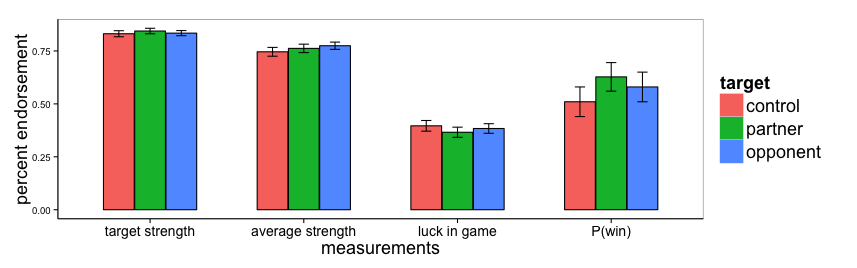
\includegraphics[width=\columnwidth]{modelE-predictions}
    \caption{Model E predictions.}
      \label{fig:modele}
\end{figure}


\section{Experiment 1}

\subsection{Methods}

Both Experiment 1 and Experiment 2 attempt to replicate the empirical results observed in KK in an online setting. The general structure of the experiments will be outlined here. 

According to the literature reviewed, motivated reasoning manifests in the difference in skill level attributed to a target player (who we call DW) that is judged based on previous performance. When the study participant is asked to assess DW's ability at a game, the participant's beliefs could be influenced by what is at stake in the game. Since both the relationship to the target and the information available about target seem to matter for motivated reasoning, our study incorporates a 2x3 condition design with a competition condition and an evidence condition. The competition condition describes the relationship between the study participant and DW, who is either a partner (P), an opponent(O), or a control (C, who is neither a partner nor an opponent). Motivated reasoning anticipates that DW will be judged as having a highest ability in the Partner condition, the lowest ability in the Opponent condition, and in-between in the control condition. 

Mirroring the conditions of KK, we employed two evidence conditions. These conditions are called  high and low evidence conditions and they determine the amount of information provided about DW. As a cover story, we tell participants that we will show them the performance of another participant in order to familiarize themselves with the workings of the game.

Since the effect is set to happen before the actual game is played, the study does not require putting participants in touch with each other.

\subsection{Materials}

We hosted the experiment at http://langcog.stanford.edu/expts/index-clean.html, and linked to it from Amazon Mechanical Turk (AMT). We recruited 145 AMT participants. Each participant was compensated with 25 cents for their participation, and one fourth of the participants were selected randomly and were awarded with a \$1 bonus (explained below).

Of the 145 subjects, we excluded 20 from the analysis due to failure to pass the competition condition manipulation check. These are participants that failed to recall their relationship with DW (e.g. someone stating that DW is his opponent when DW had been assigned as a partner).


\subsection{Procedure}

Each participant was assigned to a competition condition and to an evidence condition at random (with equal probability for each of the permutations). Before they accept to participate, participants are told that the task will take less than 10 minutes (which is the maximum time allocated to complete the task), that they will be compensated with 25 cents for participating (and that they can leave the study anytime if they so desire). Once they agreed to participate, we ask them to write down their initials (e.g. AGE) and we explain to them that they are about to play two rounds of a ``word game'' with a live partner. The game consists of two teams, each consisting of two persons: a word selector and a word unscrambler. The precise wording is:

``Each team will have a word selector and a word unscrambler. The word selector will select a word from a list of 6-letter words. The word will appear scrambled, and the word unscrambler will have 10 seconds to figure out the original word. Each team will repeat this process for ten words, and the team with the greater number of correct answers could earn up to 1 dollar, depending on the margin of difference between the two teams.''

Stating that they can earn up to 1 extra dollar if they win the game is intended to enhance the outcome dependency of the study, to increase motivation and thus enhance the potential for motivated reasoning. 

To enhance the believability of the setting, we display a dynamic ``waiting'' gif for 20 seconds while the server is ``finding players,'' followed by a 4 second wait to ``load the game''. As a cover story to present participants with evidence about DW's previous performance, we tell them that we will show them the results from a previous round in order for them to become familiar with the game. We then show DW's previous unscrambling performance by asking them to click a ``continue button'' either 2 or 8 times (depending on the evidence condition). Each time we reveal a scrambled word, the correct unscrambled word and whether or not DW answered correctly. In this study, all the words were 6 letter words, ranging from easy (banana) to extremely challenging (schism). All participants saw that DW answered each question correctly.

In the following slide participants were asked to rate DW's ``unscrambling ability'', the average ability of other Turkers (the people who do AMT tasks), the perceived ``role of luck in the game'' and the probability that their team will win. Next, a slide containing manipulation checks (e.g. ``Is DW a parter, opponent, or neither?'') and an open text field to enter open ended comments (which was intended to detect whether participants believed that they were going to play against a real human being).

Participants were then fully debriefed, and an open text field was provided for final comments about the experiment. 




\subsection{Results}

%Show: motiv-facetQuestion_mht0_n140-lines.png, or motiv-facetQuestion_mht0_n140.png.

We used an ANOVA test to analyze what accounts for the variance of the estimated strength DW. The evidence condition is significant at the p < 0.001 level, meaning that subjects were sensitive to the amount of evidence in support of DW's ability. The competition condition was not significant. When an interaction between the conditions was tested, the result was that only the evidence condition remains significant (and not the interaction variable). When other variables are included as predictors, such as the average strength of AMT participants, the role of luck in the game and the expectation of winning, the competition condition remains non-significant. A statistical significance of the competition condition as a predictor for DW strength was not found in any further analysis.

As it can be seen in (DW\_strength\_pilot.png), the mode of DW's strength as estimated by the participants is the highest possible value. Clearly the items were regarded as considerably harder than what people are capable of unscrambling in the time provided. We call this a ceiling effect, where the scale becomes less useful due to an extreme skewing of the possible answers. Numerically, the average DW strength is for the high evidence condition is 0.88 (0.84, 0.91, 95\% bootstrapped confidence intervals), and 0.80 (0.75, 0.81, 95\% bootstrapped confidence intervals).

\section{Experiment 2}

\subsection{Methods}
Since we did not find evidence of motivated reasoning in Experiment 1, we proceeded to make some changes for Experiment 2 to increase the likelihood of a non-null result. This experiment is an improvement upon Experiment 1 in various ways. First, a sense of ``team affiliation'' was cultivated throughout the experiment by making team membership much more salient. To do so, we included large banners that represented each team that were displayed when teams were assigned. The teams were called ``Red Team'' and ``Blue Team'' and it was made very explicitly that the participant was on the Red Team with another person. 

In addition the visual guide, a small ``chat box'' was designed to appear to be a communication channel between the participant and their partner. Automatically the box would first display: ``SK: ... (typing)'' quickly followed by ``SK: We can do this!'' to create the illusion that the participant's partner is a real person involved in the task and motivated to win. See team\_picture.png.

Additionally, the difficulty of unscrambling words was conveyed more realistically: by making participants engage in three practice unscrambling questions right before they were presented with DW's past performance. This in turn was also displayed in a more compelling way than in Experiment 1, showing additional information like the number of seconds that DW took to answer the question.

Since a ceiling effect for DW's strength was found in Experiment 1, the evidence was tweaked to maximize the level of ambiguity about DW's actual ability to unscramble words. Only one evidence condition was used: two questions, out of which only the easier one was solved by DW.

\subsection{Materials}

We recruited 88 participants from AMT. Those who did not pass the competition condition manipulation check were excluded from the analysis, leaving 63 compliant participants.

\subsection{Procedure}

Same as for Experiment 1 except for the changes outlined in the Methods section. The input from the participant was slightly modified: In addition to role of luck, probability of winning, etc. participants were also asked to rate ``how motivated they were to win." Finally, participants were asked to provide their age, gender, and their first language. 

\subsection{Results}

%Show: motiv2_facet-Question_n48.png

Similar to what was found in Experiment 1, ANOVA analysis showed that the competition condition was not significantly different between the competition conditions. A t-test did not show a statistically significant difference between the conditions. 


\section{Discussion}


Notice that the potential gain in this study is substantially smaller than the potential gain in the original face-to-face version (where the possible bonus for winning was \$50 dollars). This figure needs to be considered in context; the mean participant remuneration in laboratory studies is typically larger than comparable online studies by one or two orders of magnitude. So while the absolute value of the possible bonuses is very different, the relative value of the bonuses compared to the standard awards for participation are approximately equal. 

In light of the null results, it is worth examining whether motivated reasoning arises in a manner that depends on the available gains in a given context, or if the phenomenon requires a significance above certain absolute value (e.g. \$20). First, it could be that the small possible bonus (\$1) fails to invoke a sufficiently high degree of motivation in the participants for the effect to be elicited. One problem with this is that the mean self-reported ``motivation to win'' in the compliant participants of the second study is 0.84 (+0.05, -0.05, 95\% bootstrapped confidence interval) with a large minority choosing the ceiling value (1). Other measures of enhanced motivation from a \$1 bonus might be investigated in the future. The self-reported motivation is not sufficient for of the kind of motivation that leads to motivated reasoning. It would be worth considering alternative ways to measure motivation (e.g. perseverance in the face of technical problems).

Language and attention are not easily explanations of the null result. In Study 2, all participants reported being native English speakers. Thus, while we did not ask about participant's first language in Study 1, we are confident that non-native English speakers are not the source of the null result. Likewise, the number of people who failed to remember how many questions were displayed during familiarization and how many of them were answered correctly by DW is about 4 out of 5 in both studies. Excluding participants who did not satisfy this criteria from the analysis does not return significant results either. 

Finally, it could be that the evidence provided does not allow participants to construct a believable and desirable account of DW's strength in more than one way. As argued in KK, motivated reasoning arises only when people have information at their disposal with which to construct justifications for one's desired beliefs. The evidence that we presented participants in Study 1 was very similar to the evidence used in the original study: two or eight questions, all answered correctly. We obtained a ceiling effect and suspected that it might account for the null result. Even with the ceiling effect we obtained, we still saw a statistically significant difference for the evidence condition. More so, we obtained a wide spread of estimated DW strengths in Study 2 (mean of 0.57, sd of 0.20). Thus the ceiling effect is not a plausible explanation for the null results. The remaining point could be that the subject matter and difficulty of the questions we used simply do not lend themselves to motivated reasoning. Perhaps people can more readily justify their belief about a person's knowledge of American History, but cannot make a plausible story to justify motivated beliefs about ability to solve anagrams. 

\bibliographystyle{apacite}

\setlength{\bibleftmargin}{.125in}
\setlength{\bibindent}{-\bibleftmargin}

\bibliography{motivation}

\end{document}
